\subsection{Frontend Architecture and Project Structure}
The frontend of the application is a single-page application (SPA) built utilizing React and the Vite build tool. The \texttt{src/} directory is organized by architectural layer rather than by file type, ensuring each folder maintains a single, well-defined responsibility. The structure adheres to a strict one-directional dependency flow: the user-facing View layer (pages and components) depends on the State/Logic layer (context and hooks), which in turn depends on the Data layer (services) that communicates directly with the backend REST API.

\begin{figure}[H]
    \centering
    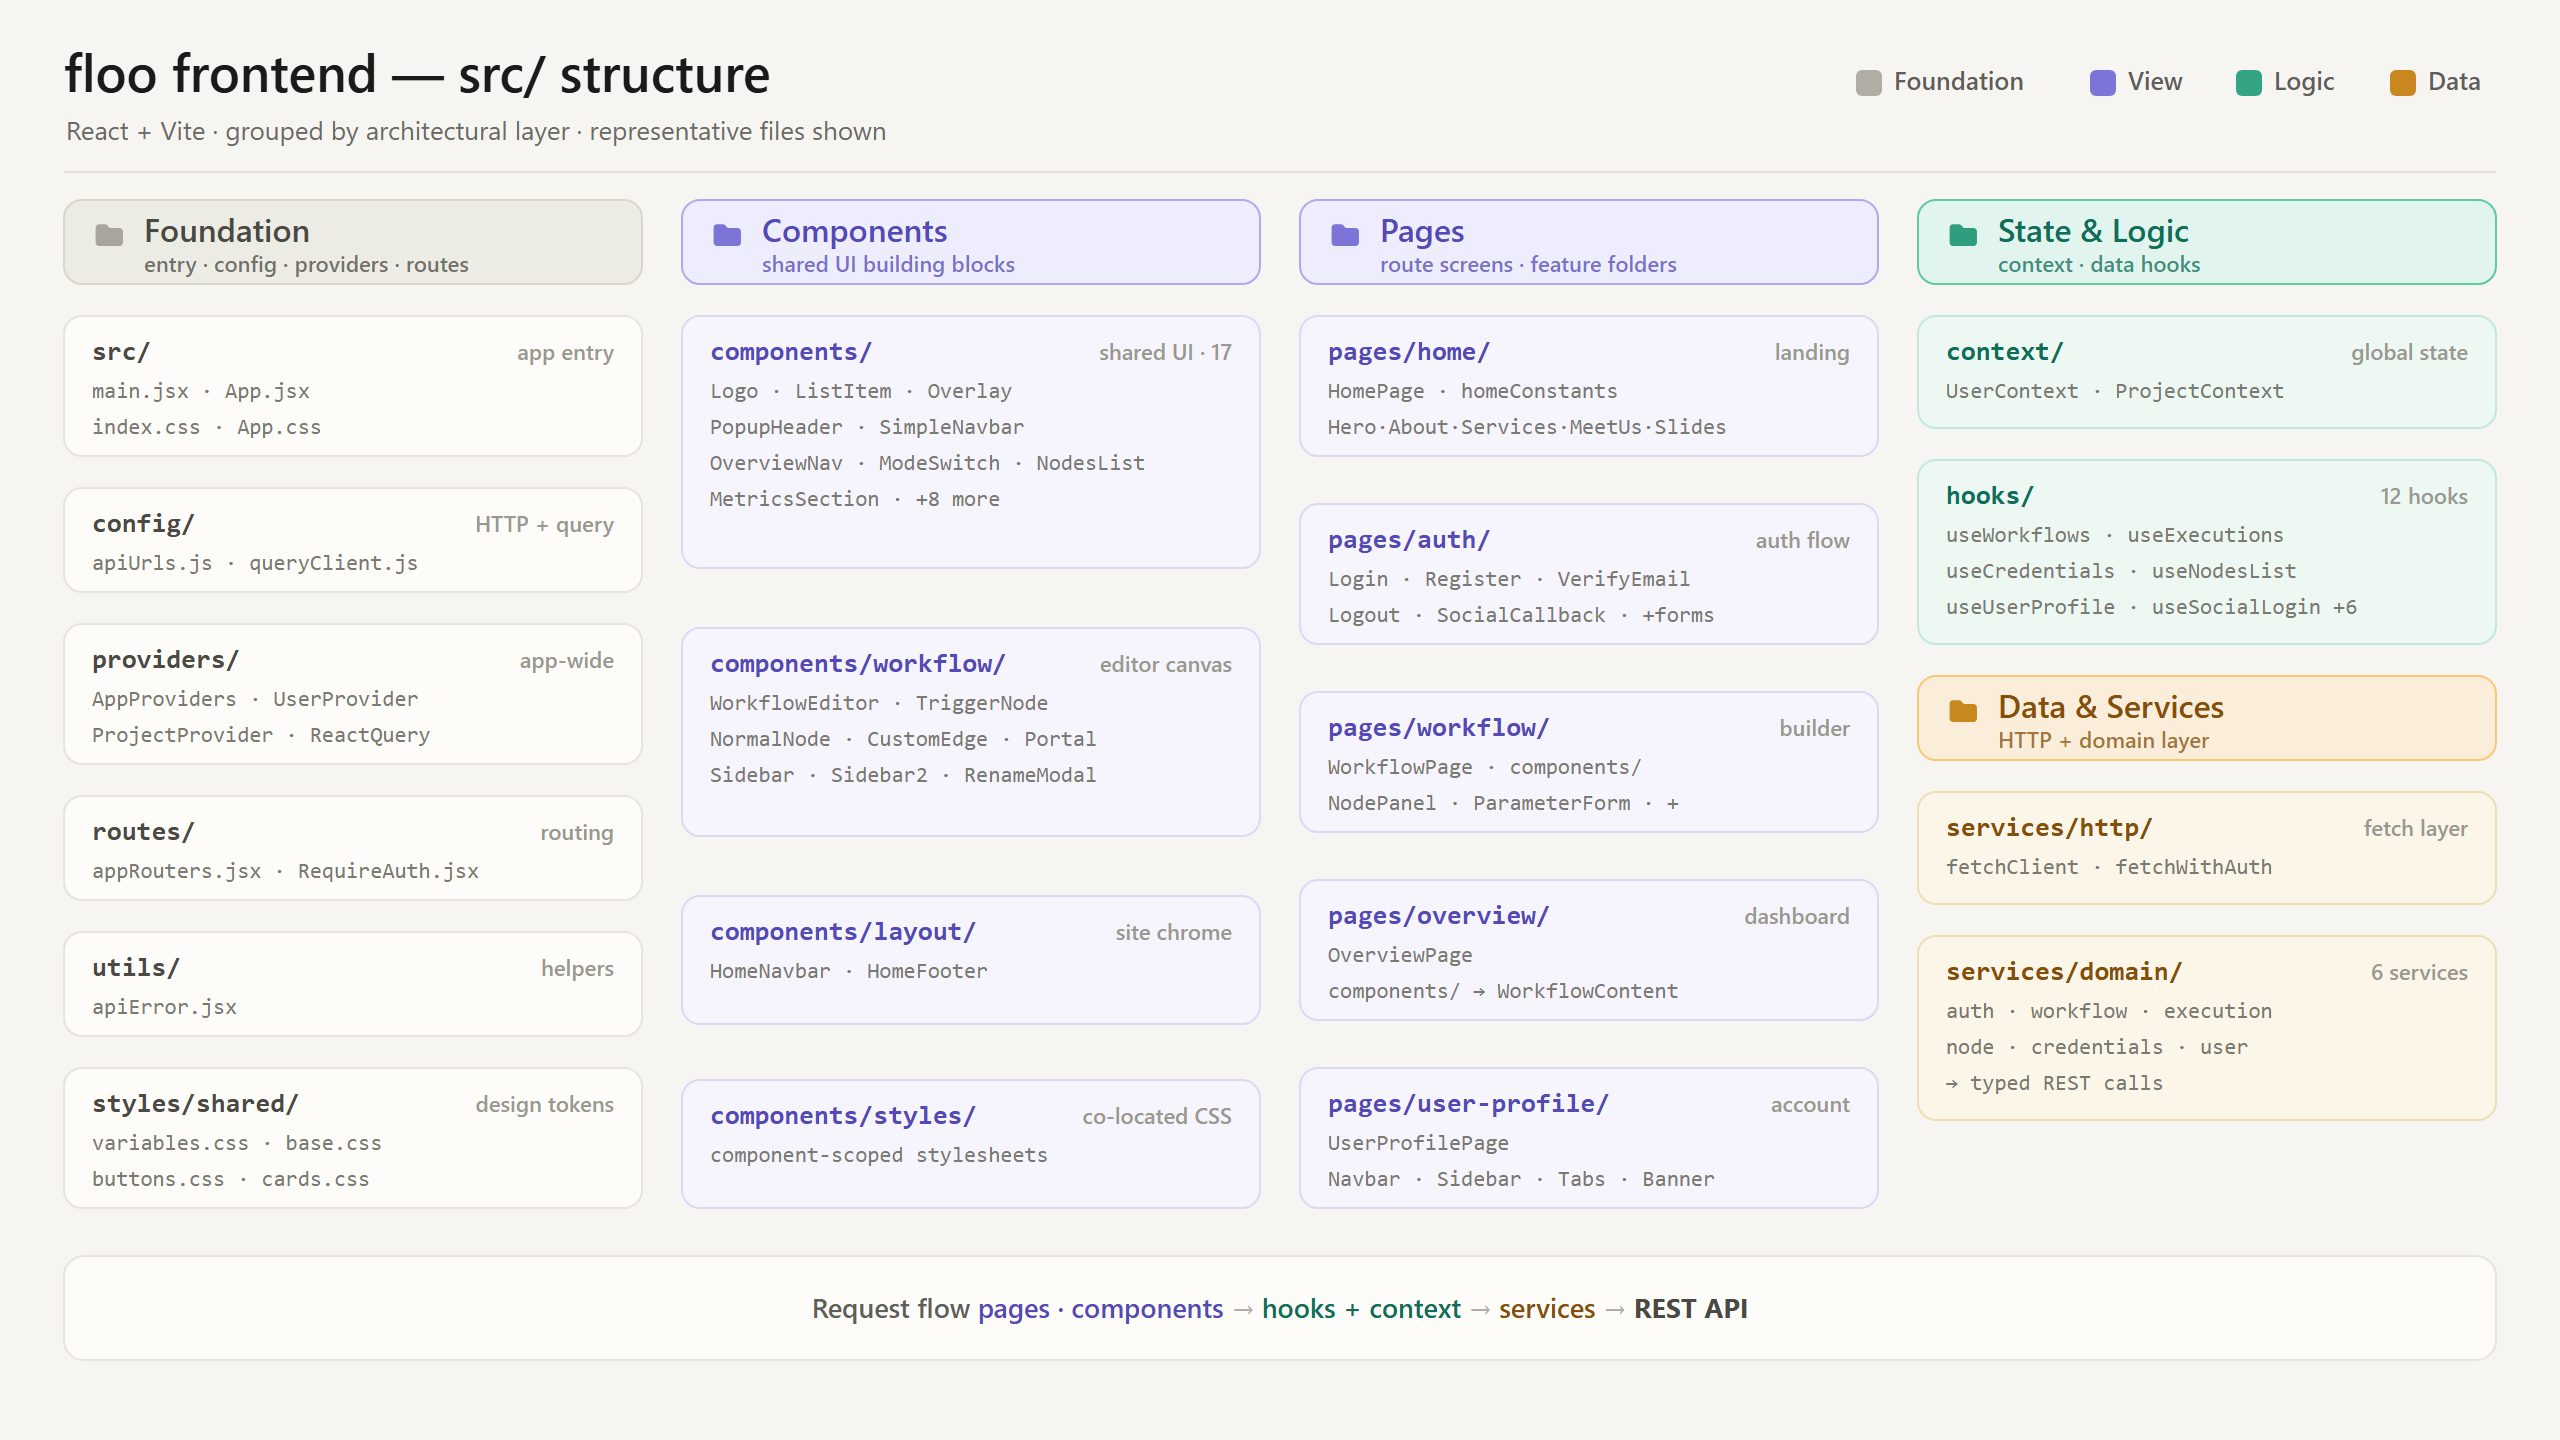
\includegraphics[width=\textwidth]{images/project-structure/project-structure1-image.png}
    \caption{Frontend Architecture and Project Structure Image}
\end{figure}

\subsubsection{Application Entry Point}

\textbf{Purpose:} Acts as the initial script executed upon application start. It bootstraps the application and hands execution control over to the routing system.

\vspace{0.2cm}
\noindent\textbf{Location:} \texttt{src/main.jsx}

\vspace{0.2cm}
\noindent\textbf{Notes:}
\begin{itemize}
    \item Utilizes React's \texttt{createRoot} to mount the application into the root HTML DOM element.
    \item Injects global stylesheets to establish baseline styling.
    \item Encapsulates the entire component tree within global providers and the router to establish application-wide state.
\end{itemize}

\subsubsection{Root Component}

\textbf{Purpose:} Serves as the top-level shell component of the application that hosts whichever page the user navigates to.

\vspace{0.2cm}
\noindent\textbf{Location:} \texttt{src/App.jsx}

\vspace{0.2cm}
\noindent\textbf{Notes:}
\begin{itemize}
    \item Renders the router's \texttt{Outlet}, functioning as the dynamic placeholder where the currently active route's page is displayed.
\end{itemize}

\subsubsection{Global Providers}

\textbf{Purpose:} Supplies application-wide state and services across the entire component tree, mitigating the need for manual "prop drilling" through nested layers.

\vspace{0.2cm}
\noindent\textbf{Location:} \texttt{src/providers/}

\vspace{0.2cm}
\noindent\textbf{Notes:}
\begin{itemize}
    \item Uses an \texttt{AppProviders} wrapper to group all individual providers into a single unified higher-order component.
    \item \textbf{UserProvider:} Manages authentication states and logged-in user data.
    \item \textbf{ProjectProvider:} Tracks the currently selected project workspace.
    \item \textbf{ReactQueryProvider:} Initializes the data-fetching and caching library context.
\end{itemize}

\subsubsection{Global State Containers}

\textbf{Purpose:} Defines the React Context objects responsible for holding shared application state, acting as the distribution channels filled by providers.

\vspace{0.2cm}
\noindent\textbf{Location:} \texttt{src/context/}

\vspace{0.2cm}
\noindent\textbf{Notes:}
\begin{itemize}
    \item Houses specific contexts such as the User and Project contexts.
    \item Allows any nested component or hook to directly subscribe to and read global values without intermediate propagation.
\end{itemize}

\subsubsection{Custom Logic Hooks}

\textbf{Purpose:} Abstracts business logic and data-fetching into reusable modules, keeping View components purely presentational and lightweight.

\vspace{0.2cm}
\noindent\textbf{Location:} \texttt{src/hooks/}

\vspace{0.2cm}
\noindent\textbf{Notes:}
\begin{itemize}
    \item Contains highly specialized hooks (e.g., \texttt{useWorkflows}, \texttt{useExecutions}, \texttt{useCredentials}).
    \item Autonomously consumes necessary context (like authentication tokens) and invokes respective API services.
    \item Manages request lifecycles, tracking active loading and error states via React Query to return ready-to-use data to the component.
\end{itemize}

\subsubsection{API Data Layer}

\textbf{Purpose:} Centralizes all network communication directly with the backend REST API, guaranteeing the rest of the application never interfaces with network requests directly.

\vspace{0.2cm}
\noindent\textbf{Location:} \texttt{src/services/}

\vspace{0.2cm}
\noindent\textbf{Notes:}
\begin{itemize}
    \item Composed of dedicated services (e.g., \texttt{WorkflowService}, \texttt{UserProfileService}) targeting specific REST endpoints.
    \item Utilizes a shared authenticated-fetch helper to automatically append user tokens and process standard JSON responses.
\end{itemize}

\subsubsection{End-to-End Execution Path}

\textbf{Purpose:} Maps the sequential runtime lifecycle of a user request traveling from the client down to the backend REST API and back.

\begin{figure}[H]
    \centering
    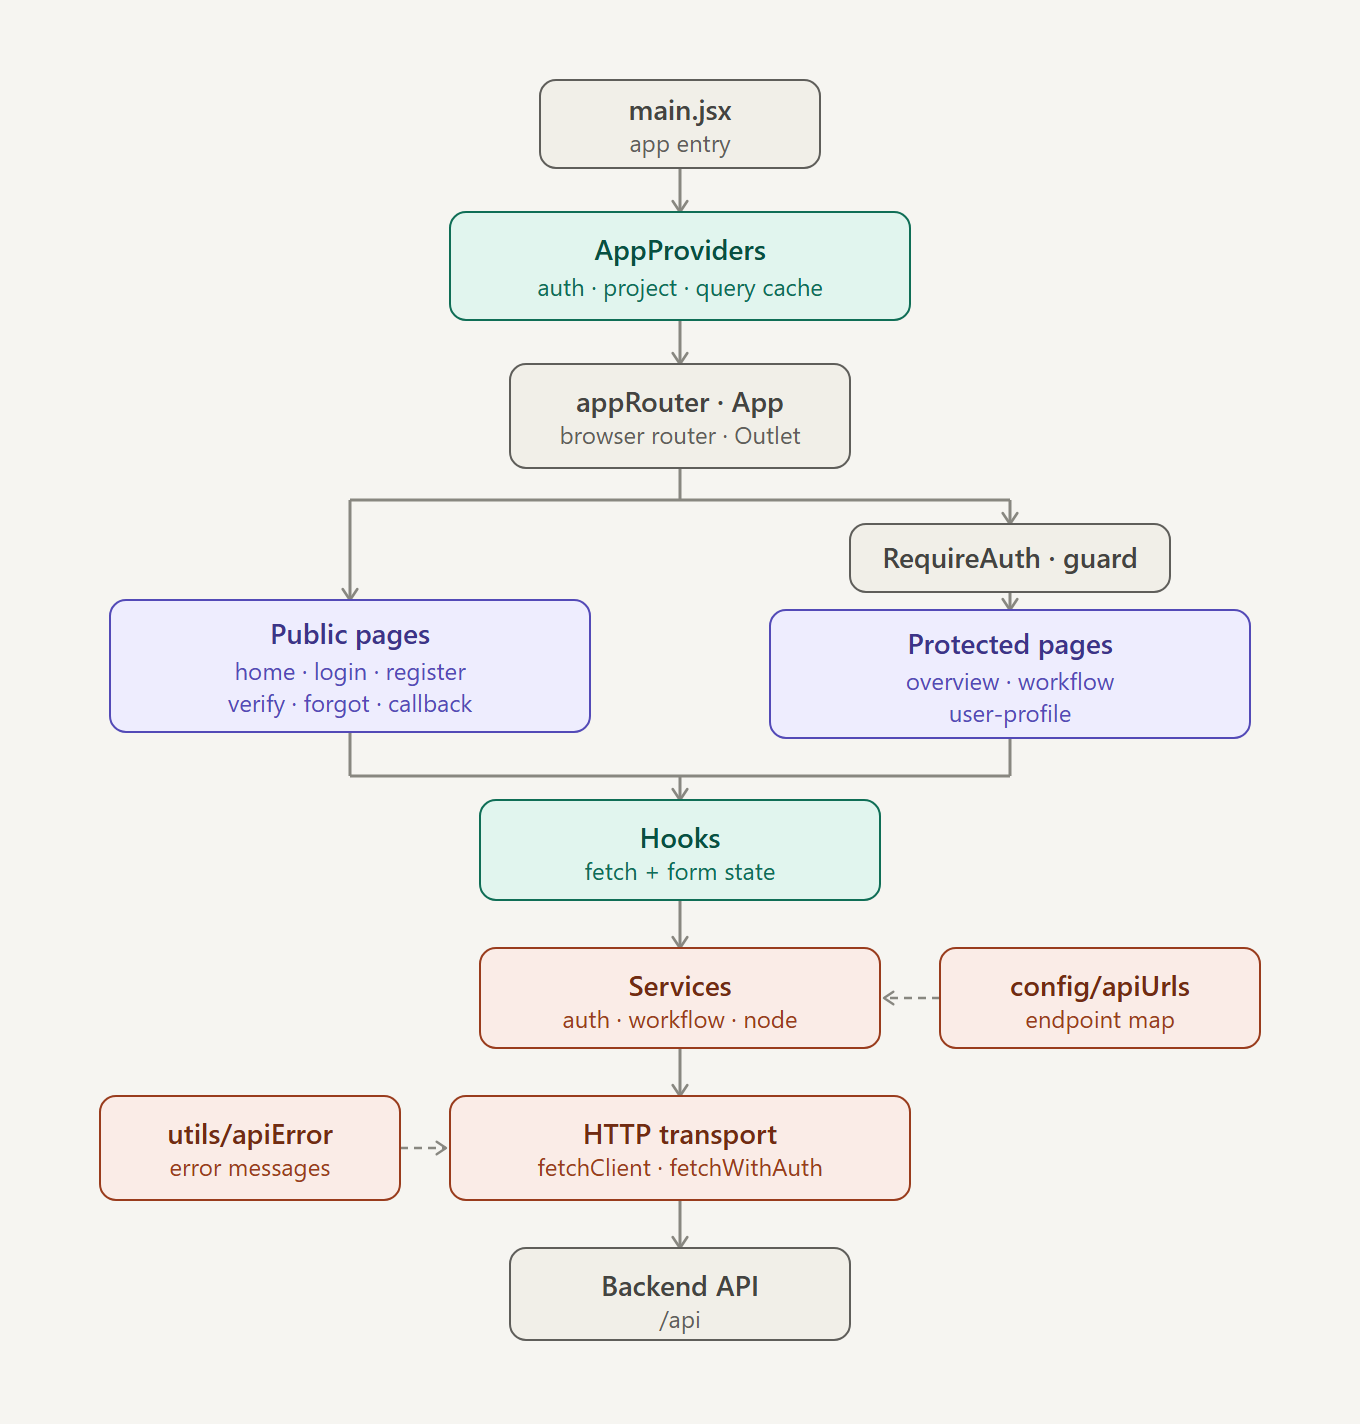
\includegraphics[width=\textwidth]{images/project-structure/project-structure2-image.png}
    \caption{Frontend Architecture and Project Structure Image}
\end{figure}

\vspace{0.2cm}
\noindent\textbf{Execution Sequence:}
\begin{enumerate}
    \item \textbf{Initialization (\texttt{main.jsx}):} The browser loads the app, executes the entry script, creates the React root, and initiates rendering.
    \item \textbf{State Wrapping (\texttt{AppProviders}):} The app is immediately enveloped by providers, guaranteeing universal access to auth state, projects, and the React Query cache.
    \item \textbf{Route Resolution (\texttt{appRouter} \& \texttt{App}):} The router evaluates the URL and injects the corresponding component into the \texttt{App} shell's \texttt{Outlet}.
    \item \textbf{Security Guarding:} Routes are split. Public pages are openly accessible, while protected pages sit behind a \texttt{RequireAuth} interceptor that force-redirects unauthorized traffic to the login screen.
    \item \textbf{Logic Invocation (Hooks):} Page components invoke a custom hook responsible for orchestrating network requests and form states rather than fetching data natively.
    \item \textbf{Service Delegation:} The active hook delegates execution to a targeted service containing the specific backend endpoint mapping.
    \item \textbf{HTTP Transport:} The service dispatches the request through a shared transport utility (\texttt{fetchClient} / \texttt{fetchWithAuth}) to securely attach the session token to the request headers.
    \item \textbf{Backend API Resolution:} The request reaches the backend \texttt{/api} endpoints; the processed response returns up the same exact pipeline to trigger client-side UI state updates.
\end{enumerate}

\vspace{0.2cm}
\noindent\textbf{Supporting Modules:}
\begin{itemize}
    \item \textbf{\texttt{config/apiUrls}:} Supplies the absolute endpoint addresses to the service layer.
    \item \textbf{\texttt{utils/apiError}:} Intercepts failed HTTP responses and translates them into human-readable error messages for the UI hooks to display.
\end{itemize}